\documentclass[12pt]{article}
\usepackage[utf8]{inputenc}
\usepackage{graphicx}
\usepackage{geometry}
\usepackage{times}
\geometry{a4paper, margin=1in}
\title{\textbf{\Huge Explorando a Arquitetura Pipeline em Processadores}}
\author{\textbf{Roger da palma}}
\date{28/05/2024}

\begin{document}

\maketitle

\section*{Introdução}

A arquitetura pipeline é uma técnica essencial na computação, permitindo aos processadores executar múltiplas instruções de forma simultânea, o que aprimora a eficiência e a velocidade do sistema. Este documento explora os diversos aspectos dessa arquitetura fascinante.

\begin{figure}[h]
\centering
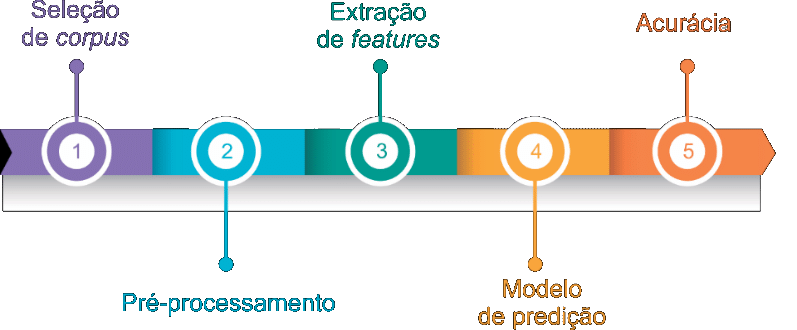
\includegraphics[width=0.8\textwidth]{fig1.png}
\caption{Estágios do pipeline de instrução em um processador.}
\label{fig:pipeline_instrucao}
\end{figure}

\section*{Processadores Pipeline}

Imagine uma linha de montagem em uma fábrica, onde cada operário executa uma tarefa específica. De maneira similar, os processadores pipeline dividem o processo de execução de instruções em várias etapas, cada uma realizada por um conjunto diferente de circuitos dentro do processador. Esta divisão permite que cada estágio do pipeline trabalhe em uma instrução diferente ao mesmo tempo, otimizando a capacidade de processamento do processador.

\begin{figure}[h]
\centering
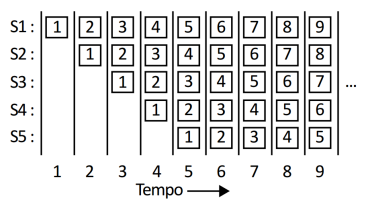
\includegraphics[width=0.6\textwidth]{fig5.png}
\caption{Estágios do pipeline de instrução em um processador.}
\label{fig:pipeline_instrucao}
\end{figure}


\section*{Pipeline de Instrução}

O pipeline de instruções, o coração do processador, é geralmente dividido em estágios como busca de instrução, decodificação, busca de dados, execução e escrita de volta. Cada estágio é responsável por uma parte específica do ciclo de vida de uma instrução, permitindo ao processador manter-se ocupado e eficiente, maximizando a taxa de execução das operações.


\section*{Desempenho do Pipeline}

A eficiência do pipeline é fundamental para o desempenho do processador, influenciada pela quantidade de estágios do pipeline e pela gestão das dependências entre as instruções. Um pipeline mais longo pode processar mais dados, mas também pode complicar a gestão de dependências e aumentar as penalidades de desempenho em casos de previsões imprecisas.

\begin{figure}[h]
\centering
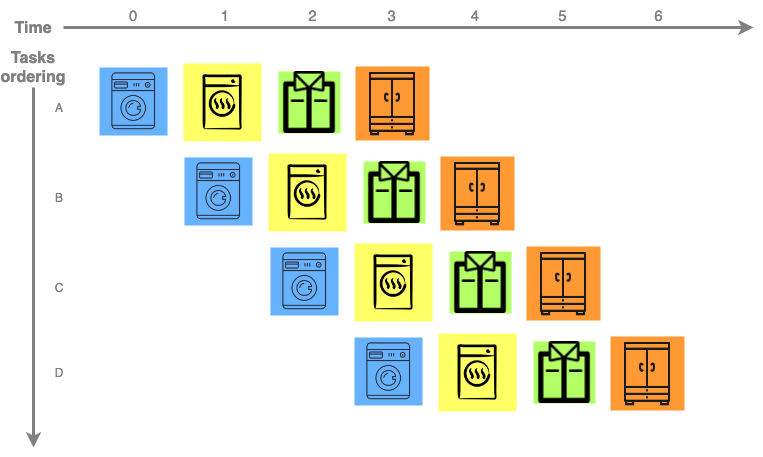
\includegraphics[width=0.6\textwidth]{fig3.png}
\caption{Estágios do pipeline de instrução em um processador.}
\label{fig:pipeline_instrucao}
\end{figure}

\section*{Hazard de Pipeline (ou Bolha de Pipeline)}

Os hazards de pipeline ocorrem quando instruções dentro do pipeline interferem umas com as outras, podendo ser estruturais, de dados ou de controle. Esses problemas podem criar "bolhas" no pipeline, períodos em que parte do pipeline fica ociosa, aguardando a resolução das dependências.

\begin{figure}[h]
\centering
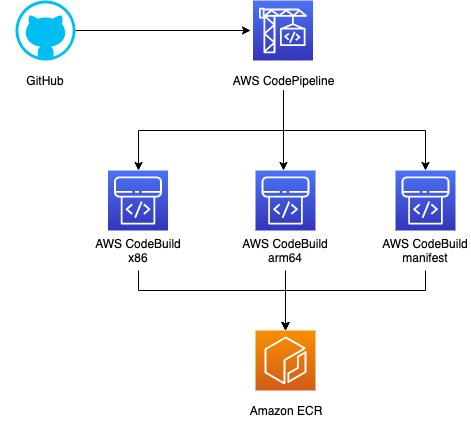
\includegraphics[width=0.7\textwidth]{fig4.jpg}
\caption{Estágios do pipeline de instrução em um processador.}
\label{fig:pipeline_instrucao}
\end{figure}


\section*{Exemplo de Processador Pipeline: Intel Core i7}

O Intel Core i7 utiliza um design de pipeline profundo e técnicas avançadas como previsão de desvios e execução fora de ordem para minimizar os hazards e otimizar o throughput, exemplificando o uso eficiente da arquitetura pipeline em processadores modernos.

\section*{Conclusão}

A arquitetura pipeline é uma parte vital dos modernos processadores, permitindo que realizem operações complexas com maior eficiência. Compreender seus componentes e desafios oferece uma visão mais clara de como as melhorias no hardware podem impulsionar o desempenho de sistemas computacionais.

\end{document}
